\setcounter{chapter}{1}
\setcounter{section}{0}
%\chapter{Introduction}
\setlength{\headheight}{12.71342pt}
\addtolength{\topmargin}{-0.71342pt}

\section{Introduction}
Fruits are complex and heterogeneous structures that comprise  a wide variety of metabolites that serve as precursors to volatile organic compounds (VOCs), such as carbohydrates, fatty acids, and pigments \cite*{A03_PanoFarias2017}. The mango fruit is no exception of this complexity and have in recent years been the focus of many studies, studying the activity of volatiles in the fruit \cite*{A04_GUO2023112779}.

\subsection{Background}
Mango is a tropical fruit which belongs to the Anacardiaceae family and is scientifically known as \textit{Mangifera} \cite*{A04_GUO2023112779}. It is popularly characterised as a sweet, juicy, aromatic fruit with a low fibre flesh \cite*{A05_Chin2019}. It is primarily cultivated in tropical and subtropical regions, where it is of significant economic importance \cite*{A05_Chin2019}. 
The annual tropical production of mango is over 46 million tons and is thereby the most produced tropical fruit after banana \cite*{A05_Chin2019, A07_Bonneau2016}. The perishable nature and susceptibility to post-harvest losses and diseases pose challenges for the mango industry, restricting the production and potential \cite*{A05_Chin2019}.

\subsection{Focus on Mango}
The mango is an important fruit crop worldwide, valued for its high nutritional content, with significant levels of fibre, vitamin C and $\beta$-carotene \cite*{A07_Bonneau2016}. However, beyond its nutritional benefits, the mango is particularly renowned for its distinctive aroma, which plays a crucial role in consumer preference and marketability \cite*{A06_Badar2016} as and indicator of quality and freshness \cite*{A05_Chin2019}.
A study by Badar et al. (2016) found that aroma is one of the most important quality attributes that influence consumer preference and acceptance of mango fruit \cite*{A06_Badar2016}. The main aroma contributors in mango are the VOCs; aldehydes, alcohols, esters and ketones \cite*{A02_Moreno2010}. Among these, 3-carene, limonene, $\beta$-pinene, acetaldehyde, ethanol and hexanal \cite*{A02_Moreno2010}. Understanding the origin and behaviour of these volatiles is therefore essential for improving fruit quality, post-harvest handling, and processing applications.

\subsection{Aim and Scope}
The aim of this report is to explore the formation, composition, and significance of VOCs in mango fruits. The main focus is on how these compounds contribute to the fruit's aroma and overall quality, both in terms of maintaining freshness and enhancing consumer appeal.
The scope includes an overview of the chemical classes and key VOCs identified in mango, the metabolic- and enzymatic pathways involved in their biosynthesis, and the influence of pre- and post-harvest conditions on their abundance. Finally, the report outlines the methods commonly applied for the extraction and identification of VOCs and their relevance for assessing fruit quality and consumer perception.

\vspace{1em}
This approach connects biochemical aroma formation with physiological and environmental factors, providing a deeper understanding of mango fruit quality from farm to table.


\section{Aroma Composition in Mango}
The complexity of aromas in mango is due to the variety of VOCs that are present in the fruit's matrix. These compounds arise from different biochemical pathways and contribute to the overall sensory experience of the fruit \cite*{A05_Chin2019}. These pathways are most prominently manifested during the ripening processes of the fruit. Also visual and textural changes occur during ripening, which further influence the perception of aroma \cite*{A01_Aguirre-Lopez_2023, A05_Chin2019}.

\subsection{Chemical Classes of Mango Aroma Compounds}
The volatile composition in fresh mango fruits has been extensively studied, revealing a diverse array with several hundred identified volatile compounds, occuring in free form in the fruit \cite*{A07_Bonneau2016}. By calculating the flavour dilution factor (FD) of the volatile compounds using gas chromatography-olfactometry (GC-O) analysis, it has been possible to identify the key aroma compounds for the odour-active fraction \cite*{A07_Bonneau2016}.

Mango aroma is primarily composed of several chemical classes. The most dominant classes is monoterpene hydrocarbons, which account for 90.2\% of the total volatile compounds in fresh mango, as illustrated in Figure \ref{fig:mango_aroma_compounds}. Other significant classes include lactones (4.1\%) and sesquiterpene hydrocarbons (3.0\%) \cite*{A07_Bonneau2016}. 

\begin{figure}
    \centering
    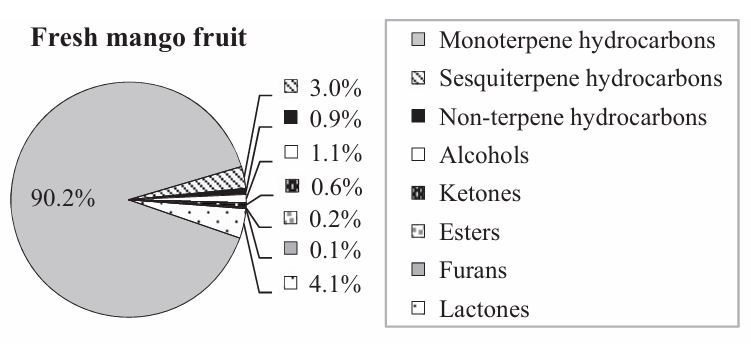
\includegraphics[width=0.8\textwidth]{Figures/fig_fresh_mango_chemical_classes.JPG}
    \caption{Distribution $[\%]$ of chemical classes of volatile compounds in fresh mango. Adapted from Bonneau et al. (2016) \cite*{A07_Bonneau2016}.}
    \label{fig:mango_aroma_compounds}
\end{figure}

\subsection{Key Aroma Compounds in Mango}
In this subsection, the key aroma compounds identified from fresh mango fruits in the study by Bonneau et al. (2016) are discussed \cite*{A07_Bonneau2016}. .

\subsubsection{Terpenes and Terpenoids}
Terpenes represent the largest class of mango aroma compounds, derived from isoprene units via the terpenoid biosynthetic pathway \cite*{A09_Barras2024}. They include both monoterpenes and sesquiterpenes, which together account for the majority of mango volatiles \cite*{A07_Bonneau2016}. Terpenes and terpenoids are found in many different natural sources, including fruits, plants, animals, microbes, and fungi. The terpenes belong to the largest class of secondary metabolites in nature and consist of five connected carbon atoms, known as isoprene units. These carbon units can be assembled in thousands of ways \cite*{B01_TerpenesTerpenoids_2018}. The terpenoids are further subcualified into five sub-groups based on the number of isoprene units they contain: monoterpenes (C10), sesquiterpenes (C15), diterpenes (C20), sesterterpenes (C25), and triterpenes (C30) \cite*{B01_TerpenesTerpenoids_2018}.

\paragraph*{Monoterpene hydrocarbons}
A total of 11 monoterpene hydrocarbons were identified as key aroma compounds in fresh mango \cite*{A07_Bonneau2016}. The most significant ones include: $\alpha$-phellandrene, $\gamma$-terpinene, $\delta$-3-carnene, $\beta$-myrcene, $\alpha$-terpinene, limonene, $\beta$-phellandrene, and $\alpha$-terpineolene. 

\vspace{1em}
Monoterpenes are the smallest molecules in the isoprenoid family with conserved hydrocarbons \cite*{A09_Barras2024}. They share the formula $C_{10}H_{16}$ and over 400 different chemical structures has been classified as such \cite*{A09_Barras2024}. The key monoterpene hydrocarbons identified in mangos are reported to have significant impact on the overall odorants \cite*{A07_Bonneau2016}.

\paragraph*{Sesquiterpene hydrocarbons}
Compared to monoterpenes, sesquiterpenes are larger molecules with the formula $C_{15}H_{24}$. In mango fruit, the study by Bonneau et al. (2016) identified four key sesquiterpene hydrocarbons, including: $\alpha$-gurjunene, $\alpha$-copaene, $\beta$-caryophyllene, and $\alpha$-caryophyllene \cite*{A07_Bonneau2016}.


\subsubsection{Alcohols and Aromatic Alcohols}
Alcohols and aromatic alcohols are, like terpenes and terpenoids, major contributors to the key aroma of mango, though they differ in chemical structure and biosynthetic origin. A study by Singh et al. (2010) highlighted the role of alcohol dehydrogenase (ADH) in the enzymatic reduction of aldehydes leading to the formation of these compounds \cite*{A10_Singh2010}.

\vspace{1em}
A total of nine alcohols were identified as volatile compounds in \textit{Kent} fresh mango \cite*{A07_Bonneau2016}. Among these compounds, 1-butanol was quantified as one of the key aroma contributors. Other identified alcohols include 3-methyl-1-butanol, 2-decanol, and 1-hexanol. Many compounds, such as 2-methyl-1-propanol did not appear in the fresh \textit{Kent} mango, but increased significantly during drying \cite*{A07_Bonneau2016}.

\subsubsection{Aldehydes and Aromatic Aldehydes}
Aldehydes are volatile compounds primarily formed through the oxidation of unsaturated fatty acids, such as $\alpha$-linolenic acid, via the lipoxygenase (LOX)-hydroperoxide lyase (HPL) pathway. These reactions generate C$_6$ and C$_9$ aldehydes, often referred to as green leaf volatiles, which are associated with fresh and grassy notes in the mango fruit aroma \cite*{A11_Sivankalyani2017}. In mango, this pathway becomes particularly active under chilling stress, leading to increased levels of compounds such as 1-hexanal, (\textit{E})-2-hexenal, and (\textit{Z})-3-hexenal before visible quality loss occurs.

\vspace{1em}
In the fresh \textit{Kent} mango, a total of one aldehyde, hexanal, was identified as key aroma compounds \cite*{A07_Bonneau2016}. While not detecable in the fresh fruit, the study did identify a total of six aldehydes post-drying, include hexanal, (\textit{E,E})-2,4-heptadienal, nonanal, and (\textit{E,Z})-2,4-heptadienal \cite*{A07_Bonneau2016}.

\subsubsection{Lactones}
Lactones are VOCs that quantitatively represents a smaller fraction of the mango aroma profile compared to terpenes and terpenoids. They are nonetheless important contributors to the overall sensory experience of the fruit, and make up two times the quantitative amount of alcohols, ketones, esters, and furans combined \cite*{A14_Silva2021, A07_Bonneau2016}. Lactones are cyclic esters formed through the intramolecular esterification of hydroxy acids. In mango, they are primarily derived from the oxidation and subsequent cyclization of fatty acids during the ripening process \cite*{A13_ElHadi2013}.

\vspace{1em}
A total of five lactones were identified as volatile compounds in fresh mango, in the study by \textcite*{A07_Bonneau2016}. Among these compounds, the most significant constituent in the fresh fruit was $\gamma$-butyrolactone. Other lactones detected includes: $\alpha$-methyl-$\gamma$-bytyrolactone, $\gamma$-hexalactone, $\delta$-hexalactone, and $\delta$-ocatlacetone \cite*{A07_Bonneau2016}.

\subsubsection{Minor Volatile Compounds: Ketones, Esters, and Furans}
Ketones, esters, and furans are present in much smaller amounts compared to terpenes and terpenoids, but still contribute to the complexity of mango aroma \cite*{A07_Bonneau2016}. Ketones are important volatile compounds that can be identified in exotic fruits such as mango, e.g. 1-octen-3-ona, which provides a mushroom aroma \cite*{A01_Aguirre-Lopez_2023}. Esters are associated with fruity and sweet nuances, whereas the furans provide the mango fruit with mild caramel-like notes. Despite low abundance of these three classes of compounds, they may enhance the overall balance of aroma perception in fresh mango \cite*{A13_ElHadi2013}.

\subsection{Variation in Aroma Profiles Among Mango Varieties}
The volatile composition of mango (\textit{Mangifera indica} L.) varies substantially among cultivars, reflecting genetic differences and environmental influences on fruit metabolism and ripening \cite*{A01_Aguirre-Lopez_2023}. Comparative analyses of multiple mango varieties have shown that the abundance and composition of key aroma compounds differ significantly across cultivars, leading to distinct sensory profiles \cite*{A01_Aguirre-Lopez_2023,A02_Moreno2010}. 

\vspace{0.5em}
A recent study by \textcite{A16_Tandel2023} investigated sixteen Indian mango cultivars, revealing notable differences in their volatile profiles. Cultivars such as \textit{Alphonso}, \textit{Kesar}, and \textit{Ratna} were characterised by high levels of terpenes, whereas \textit{Amrapali} was dominant in esters \cite*{A16_Tandel2023}. Within the terpene class, \textit{allo-ocimene} and $\beta$-ocimene were frequently dominant, while the presence of butanoic acid derivatives contributed to the sweeter aroma of ester-rich cultivars \cite*{A16_Tandel2023}. 

\vspace{0.5em}
\textcite{A13_ElHadi2013} further distinguished the aroma profiles of mango cultivars according to their geographical origin. New World varieties, such as \textit{Haden}, \textit{Irwin}, and \textit{Tommy Atkins}, were typically dominated by terpene hydrocarbons—especially $\delta$-3-carene—whereas Old World cultivars contained higher proportions of esters, alcohols, and ketones, resulting in sweeter and fruitier profiles \cite*{A13_ElHadi2013}. 

\vspace{0.5em}
As discussed by \textcite{A16_Tandel2023}, previous studies comparing Chinese cultivars \textit{Tainong} and \textit{Jinmang} found high levels of $\beta$-ocimene, myrcene, and $\alpha$-terpinolene, which significantly contributed to their aroma profiles. These results aligned with \textcite{A15_Xie2023}, who also reported terpenes as a dominant volatile class in \textit{Jinmang}. In a separate comparison of \textit{Tainong} and \textit{Hongyu}, \textcite{A15_Xie2023} observed that \textit{Tainong} had higher levels of terpenes and aldehydes, producing a grassy aroma, while \textit{Hongyu} exhibited higher ester content, leading to a more fruity and sweet aroma.


\section{Biochemical Pathways of Aroma Compound Formation}
VOCs are low-molecular-weight molecules with functional groups such as alcohols, esters, ketones, aldehydes, and terpenes \cite*{A01_Aguirre-Lopez_2023,B01_TerpenesTerpenoids_2018}. These compounds are synthesised through metabolic and enzymatic reactions during maturation and ripening, and significantly impacts the fruits aroma profile \cite*{A01_Aguirre-Lopez_2023}. VOC profiling is therefore an important indicator of fruits quality, cultivar differentiation, and ripeness \cite*{A01_Aguirre-Lopez_2023}. 

\vspace{1em}
The study of VOCs is known as \textit{volatilomics}, which investigates the biosynthesis and metabolic pathways of aroma compounds \cite*{A01_Aguirre-Lopez_2023}. The biosynthesis of VOCs in fruits is based on three major pathways: the amino acid derivative pathway, the fatty acid derivative pathway, and the terpenoid pathway \cite*{A13_ElHadi2013}. These pathways will be described in detail below. Once the basic molecular forms are synthesised, enzymatic reactions, such as hydroxylation, acylation, methylation, oxidation-reduction, and ring closure, enhance volatility and molecular diversity \cite*{A13_ElHadi2013}.


\subsection{Enzymes Involved in Aroma Biosynthesis}
The diversity of VOCs in mango arises from enzymatic reactions that modify basic molecular structures, e.g. hydroxylation, acylation, methylation, oxidation-reduction, and ring closure \cite*{A13_ElHadi2013}. ADH plays a key role in converting aldehydes to alcohols and supplies substrates for ester synthesis. Mangoes expresses multiple ADH isoforms (MiADH1-3) that are differentially regulated during ripening \cite*{A10_Singh2010}. Other enzymes which contributes to the aroma formation includes methionine $\gamma$-lyase and 3-ketoacyl-CoA thiolase B, which are active in amino-acid- and fatty-acid-derived pathways \cite*{A05_Chin2019}. In the fatty acid pathway, LOX and HPL cooperates with ADH to produce $C_6$ and $C_9$ volatiles, whereas terpene synthases (TPSs) catalyses the cyclisation of prenyl diphosphate precursors in the terpenoid pathway \cite*{A13_ElHadi2013}.


\subsection{Amino Acid Derivative Pathway}
The Amino Acid Derivative Pathway is responsible for synthesizing the fruits characterised flavour and aroma compounds \cite*{A13_ElHadi2013}. Amino acids, such as alanine, valine, leucine, isoleucine, phenylalanine, and aspartic acid, serves as direct precursors for these pathways, forming a variety of compounds including alcohols, carbonyls, acids, and esters \cite*{A13_ElHadi2013}. The biosynthesis typically starts with a deamination or transamination reaction that produces the corresponding $\alpha$-keto acid \cite*{A13_ElHadi2013}. Subsequent steps follows, including decarboxylation, reduction, oxidation, and/or esterification, to produce the volatile compounds \cite*{A13_ElHadi2013}, e.g. branched chain volatiles, which often are derived from leucine, isoleucine, and valine \cite*{A05_Chin2019}.


\subsection{Fatty Acid Derivative Pathway}
The fatty acid derivative pathway is a major source of aroma volatiles in fruits. The pathway produces straight-chain alcohols, aldehydes, ketones, esters, and lactones \cite*{A13_ElHadi2013}. There are mainly three processes involved in the fatty acid derivative pathway: $\alpha$-oxidation, $\beta$-oxidation, and the LOX pathway \cite*{A13_ElHadi2013,A16_Tandel2023}. The $\beta$-oxidation process shortens fatty acids by removing $C_2$ units (acetyl-CoA), forming precursors for ester synthesis \cite*{A13_ElHadi2013}. The LOX pathway converts polyunsaturated fatty acids such as linoleic and linolenic acid into $C_6$ and $C_9$ aldehydes and alcohols via HPL and ADH \cite*{A13_ElHadi2013}. Compounds like hexanal and nonanal are formed by linolenic and oleic acid degradation, and hydroxylated intermediates can undergo spontaneous lactonization to form lactones such as $\gamma$-butyrolactone \cite*{A07_Bonneau2016,A14_Silva2021}.


\subsection{Terpenoid Pathway (MEP and MVA Pathways)}
Terpenoids represent the largest class of plant secondary metabolites, the two primary groups are monoterpenes and sesquiterpenes \cite*{A04_GUO2023112779, A02_Moreno2010, A09_Barras2024}. They all share the $C_5H_8$ isoprenoid unit and are derived from the universal precursors isopentenyl diphosphate (IPP) and dimethylallyl diphosphate (DMAPP), and are synthesised by two distinct routes: the cytosolic mevalonic acid (MVA) pathway, and the plastidial methylerythritol-4-phosphate (MEP) pathway \cite*{A09_Barras2024,A13_ElHadi2013}. MVA starts from acetyl-CoA, whereas MEP uses pyruvate and glyceraldehyde-3-phosphate (G3P) as precursors \cite*{A09_Barras2024}. These pathways happens simultaneously in different cellular compartments, enabling an exchange of intermediates \cite*{A09_Barras2024}. Subsequently, IPP and DMAPP are joined together by prenyltransferases which produces geranyl pyrophosphate (GPP) and farnesyl pyrophosphate (FPP) \cite*{A09_Barras2024,A13_ElHadi2013}. TPSs then catalyses the cyclisation into different terpene skeletons that defines the mango aroma \cite*{A09_Barras2024,A13_ElHadi2013}.


\section{Environmental and Genetic Factors Influencing Aroma Production}
The aroma profile of fruit is complex and determined by a combination of both genetics and environmental factors \cite*{A13_ElHadi2013,A16_Tandel2023}. The composition and concentration of VOCs are specific to the fruit species and across cultivars \cite*{A13_ElHadi2013,A16_Tandel2023}. Variations among mango cultivars, for example, demonstrate that genetic background defines the abundance of specific volatile classes (e.g., some are monoterpene-dominant, while others has high levels of esters, fatty acids, or sesquiterpenes) \cite*{A16_Tandel2023}.


\subsection{Pre-harvest Factors}
Pre-harvest conditions significantly influence the final volatile composition \cite*{A13_ElHadi2013}. Environmental conditions such as climate (temperature and humidity) and geographic region (sunlight, precipitation, and fertilisation) can modulate VOC quantity in plants \cite*{A01_Aguirre-Lopez_2023,A16_Tandel2023}. These factors affect crop growth and aroma quality, including flavour and texture \cite*{A13_ElHadi2013}. 


\subsection{Post-harvest Factors}
The stage of maturity and ripening is a critical post-harvest factor since VOCs are released during the maturation processes \cite*{A01_Aguirre-Lopez_2023,A13_ElHadi2013}. In climacteric fruits like mango, ripening is associated with an increase in ethylene production and subsequent synthesis of aromatic volatiles \cite*{A05_Chin2019}. In mango, the expression of key aroma genes, such as ADH, is regulated by hormones like ethylene and Abscisic Acid (ABA) at the initial stages of ripening \cite*{A10_Singh2010}. Furthermore, storage temperature has a significant impact on the volatile profile \cite*{A13_ElHadi2013}. Storing mangoes at sub-optimal temperatures (e.g.5\textdegree C) induces chilling stress, which results in a reduced formation of desirable aroma compounds such as monoterpenes, while it simultaneously increases $C_6$ and $C_9$ aldehydes \cite*{A11_Sivankalyani2017}.


\subsection{Processing Implications on Aroma Retention}
Processing methods, particularly drying, results in a significant loss of aroma compounds \cite*{A07_Bonneau2016}. A study by \textcite{A07_Bonneau2016} on drying \textit{Kent} mango fruit showed a total volatile loss of approximately 58.8\% \cite*{A07_Bonneau2016,A16_Tandel2023}. This decline is primarily attributed to evaporation and thermal degradation of compounds such as monoterpenes, sesquiterpenes, and lactones \cite*{A07_Bonneau2016}. However, pretreatment techniques like osmotic dehydration (DO) has shown to help decrease these losses and aid in the conservation of volatile compounds \cite*{A02_Moreno2010}. It was proposed that sugar impregnation blocked the exit of internal gases during subsequent drying \cite*{A02_Moreno2010}. Some compounds, such as hexanal and nonanal, showed a post-drying increase possibly due to the degradation of unsaturated fatty acids \cite*{A07_Bonneau2016}.


\section{Analytical Techniques for Aroma Compound Identification}
\subsection{Extraction and Analysis Methods}
The most common technique for sampling volatile compounds in fruits is Solid Phase Microextraction (SPME) \cite*{A01_Aguirre-Lopez_2023}. SPME is highly favored because it is solvent-free, fast, sensitive, and requires minimal sample manipulation by reliably collecting analytes from the headspace (HS) \cite*{A01_Aguirre-Lopez_2023,A03_PanoFarias2017}. The technique typically utilizes adsorbent fibers composed of materials such as DVB, CAR, PDMS, and PA to capture the volatile compounds \cite*{A01_Aguirre-Lopez_2023}. When extracted, the Gas Chromatography coupled with Mass Spectrometry (GC-MS) is used, which separates molecules and identifies them via mass detection \cite*{A01_Aguirre-Lopez_2023}. Other used methods include Liquid-Liquid Extraction (LLE) for non-polar VOCs \cite*{A01_Aguirre-Lopez_2023}, Solvent Assisted Flavour Evaporation (SAFE) for preparing aroma extracts of the original product \cite*{A01_Aguirre-Lopez_2023}, and Single Drop Microextraction (SDME) for miniaturized analysis \cite*{A03_PanoFarias2017}.


\subsection{Quantification and Sensory Evaluation}
Sensory analysis is a crucial aspect. Odour and aroma are quality attributes directly linked to consumer acceptance \cite*{A01_Aguirre-Lopez_2023}. To quantify the sensory impact, the Odor Activity Value (OAV) estimates odor potency by calculating the ratio between a compound's concentration and its odor detection threshold \cite*{A01_Aguirre-Lopez_2023,A07_Bonneau2016}. Similarly, Aroma Extract Dilution Analysis (AEDA) can rank the perception of compounds which are important to the overall aroma via the flavor dilution (FD) factor \cite*{A01_Aguirre-Lopez_2023,A07_Bonneau2016}. Specialized techniques combines analysis with human perception, such as GC-Olfactometry (GC-O), which routes the column effluent to a "sniffing port" for sensory evaluation by a trained panel \cite*{A01_Aguirre-Lopez_2023}. Furthermore, Multivariate Data Analysis, such as Multiple Correspondence Analysis (MCA), is used to explore statistical correlations between molecules, aromas, and fruits \cite*{A01_Aguirre-Lopez_2023,A15_Xie2023}.


\section{Comparative Perspective}
Mango aroma varies significantly across cultivars, geography, and processing, indicating both genetic and environmental influences on volatile biosynthesis \cite*{A13_ElHadi2013,A16_Tandel2023}. Indian cultivars showed differences like \textit{Alphonso}, \textit{Kesar}, and \textit{Ratna} which often are terpene-dominant, while other cultivars exhibited different major components, such as \textit{Neelum} which had high levels of sesquiterpenes (74.80\%) \cite*{A16_Tandel2023}. Geographical factors also showed significant variations. New World varieties (\textit{Haden} and \textit{Tommy Atkins}) were dominated by terpene hydrocarbons, while Old World mangoes contained higher proportions of esters, alcohols, and ketones \cite*{A13_ElHadi2013}. Similarly, analysis confirmed that \textit{Tainong} expressed grassy notes due to high terpene and aldehyde content, while \textit{Hongyu} was rich in esters and were perceived as fruity and sweet \cite*{A15_Xie2023}.

\vspace{1em}
Ripening and post-harvest handling significantly impacts the aroma profiles. During maturation, ethylene activation enhances the synthesis of aromatic volatiles, including terpenes and esters derived from pathways involving ADH \cite*{A10_Singh2010}. Conversely, chilling stress (e.g., storage at 5\textdegree C) compromises aroma quality by suppressing monoterpenes and increasing the concentration of stress-related $C_6$ and $C_9$ aldehydes and alcohols \cite*{A11_Sivankalyani2017}. Drying \textit{Kent} mangoes greatly reduces the total volatile content, mainly through the loss of terpenoids, but compounds like lactones and esters may be retained or enriched, altering the sensory balance \cite*{A07_Bonneau2016}. Techniques like osmotic dehydration has been proposed to help mitigate these losses \cite*{A02_Moreno2010}.

\vspace{1em}
The variation observed in aroma studies is often attributed to the analytical choices, as the volatile profile is highly sensitive to the method used \cite*{A13_ElHadi2013}. Techniques such as SPME, SDME, and SAFE capture different classes of compounds from the fruit headspace \cite*{A01_Aguirre-Lopez_2023,A07_Bonneau2016}. Crucially, GC-O, often utilizing flavor dilution analysis, identifies compounds based on their potent sensory impact, such as a high OAV, rather than only their chemical abundance recorded by GC-MS \cite*{A01_Aguirre-Lopez_2023,A07_Bonneau2016}.


\section{Conclusion}
Mango aroma complexity stems from the interaction of hundreds of VOCs, predominantly monoterpene hydrocarbons, which originate primarily from three core biosynthetic routes: the Terpenoid pathway, the Fatty Acid Derivative pathway, and the Amino Acid Derivative pathway.

\vspace{1em}
The specific aroma profile is highly influenced by the cultivars genetic background, leading to significant differences between terpene-dominant New World cultivars and ester/alcohol-rich Old World varieties. This inherent chemistry is critically influenced by environmental and post-harvest factors. Ripening promotes the synthesis of aromatic volatiles, while stresses, such as cold storage (5\textdegree C), lead to less formation of monoterpenes and an increase in both $C_6$ and $C_9$ aldehydes from the oxidation of $\alpha$-linolenic acid. Furthermore, processing methods like drying, causes significant losses of volatile compounds, approximately 58.8\%, although pre-treatment strategies like osmotic dehydration can mitigate the aroma decrease.

\vspace{1em}
Accurate characterization of the aroma profiles relies on analytical tools, primarily SPME extraction coupled with GC-MS, complemented by sensory techniques like GC-O and OAV to identify the few odor-active compounds that define consumer perception. Comprehensive understanding of these biochemical and environmental factors are essential for the mango industry to optimize post-harvest handling and select cultivars that guarantee specific, consumer-desirable aroma traits. Future research should aim to combine volatilomics with genetic data, thereby linking the key synthesis enzymes like ADH, TPSs, and LOX to cultivar-specific aroma formation.
